% !TEX root = msc_thesis.tex

\begin{figure}[tb]
	\centering
	\begin{subfigure}[b]{1.0\textwidth}
		\centering
		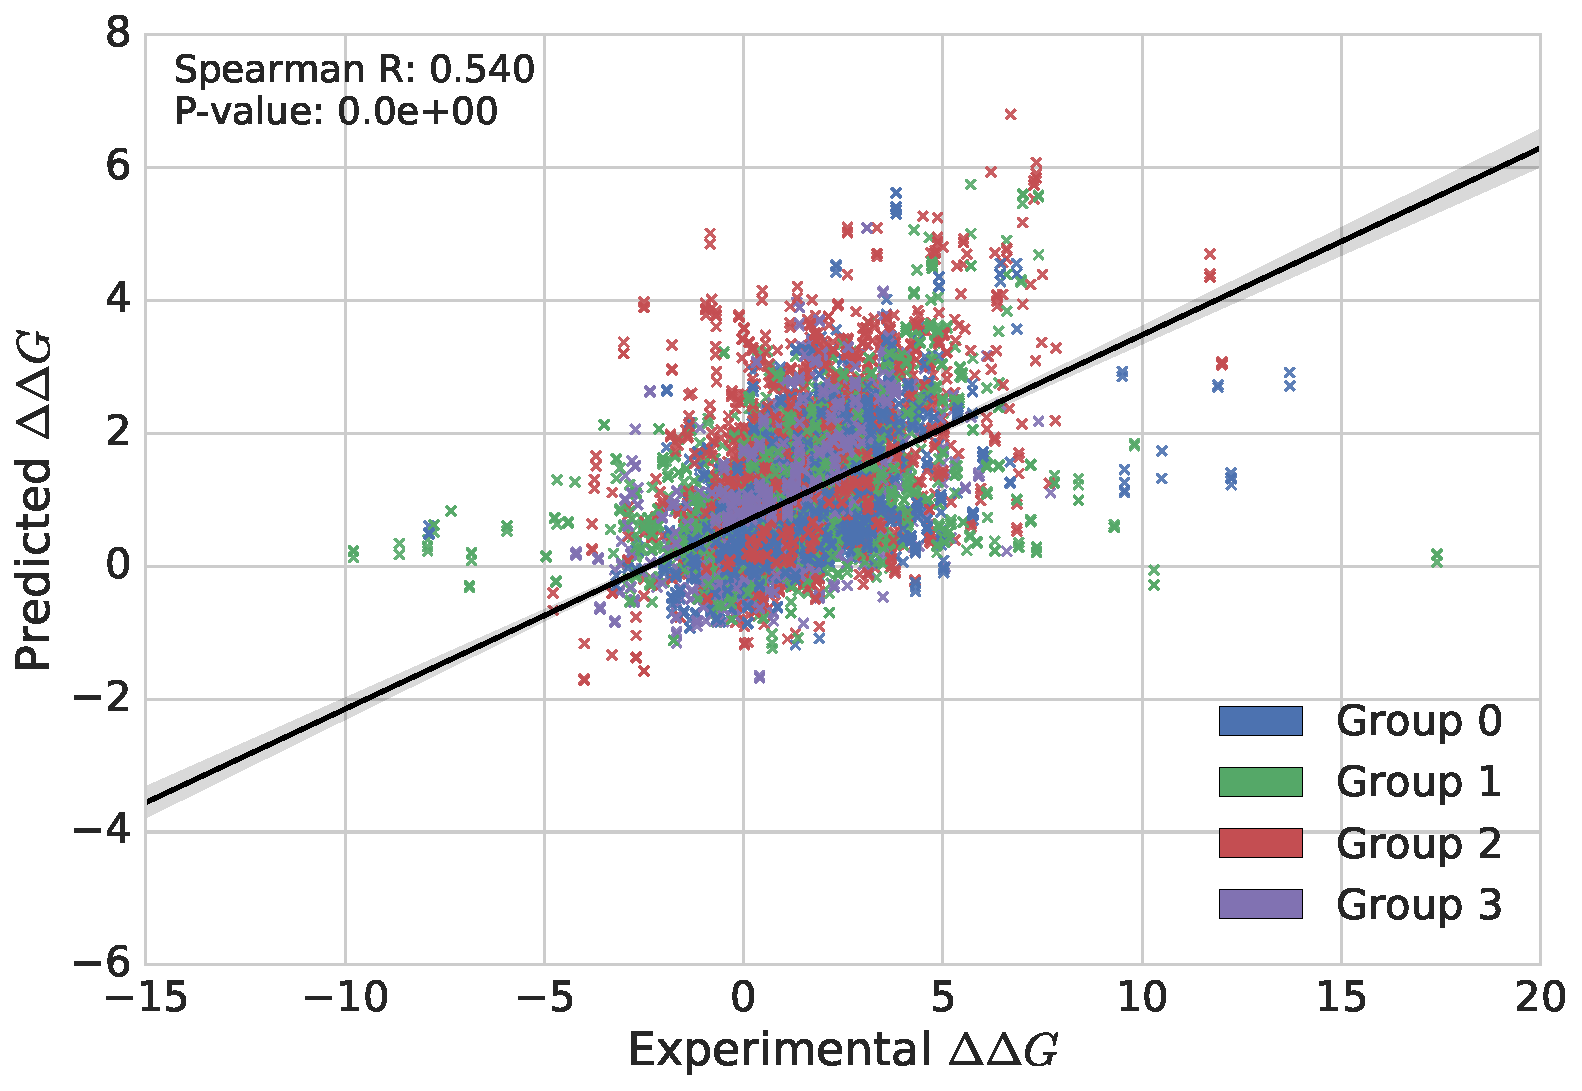
\includegraphics[width=0.6\linewidth]{static/elaspic_training_set/validation/crossvalidation_performance_core.pdf}
		\caption{
			Performance of the ELASPIC core predictor on the training dataset, evaluated using four-fold cross-validation.
			Colours indicate different cross-validation bins.
		}
		\label{fig:crossvalidation_performance_core}
		\vspace*{10mm}
	\end{subfigure}
	\begin{subfigure}[b]{1.0\textwidth}
		\centering
		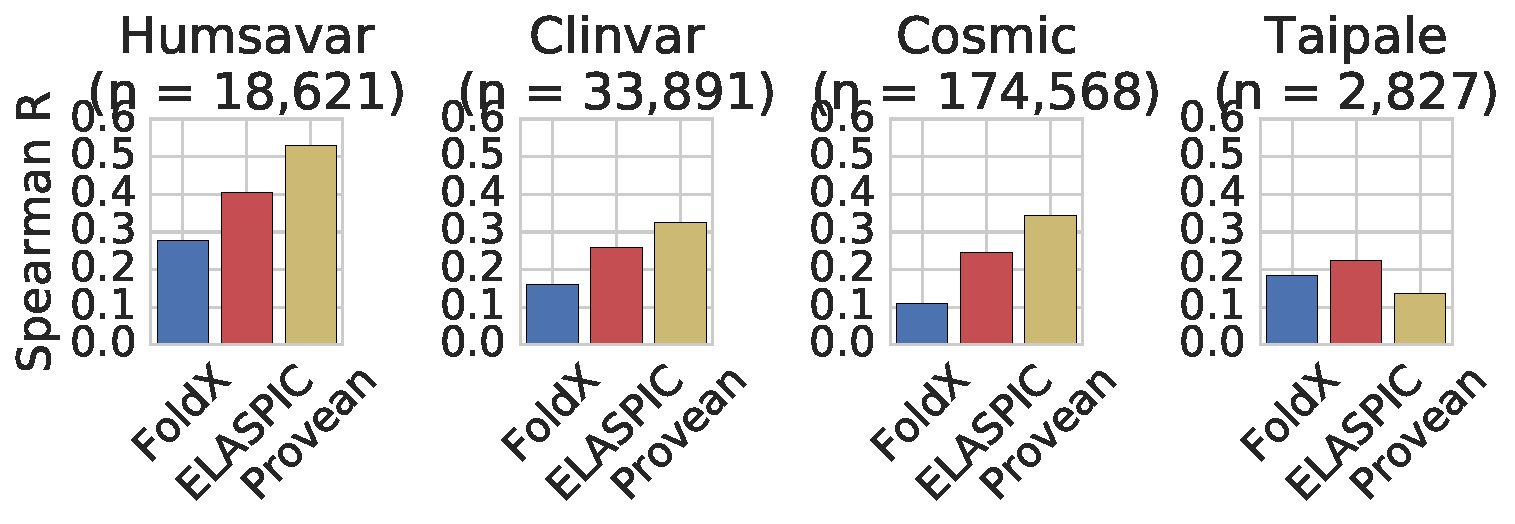
\includegraphics[width=0.8\textwidth]{static/elaspic_training_set/validation/validation_performance_core.pdf}
		\caption{
			Performance of the ELASPIC core predictor, FoldX and Provean on the validation datasets.
		}
		\label{fig:validation_performance_core}
		\vspace*{10mm}
	\end{subfigure}
	\begin{subfigure}[b]{1.0\textwidth}
		\centering
		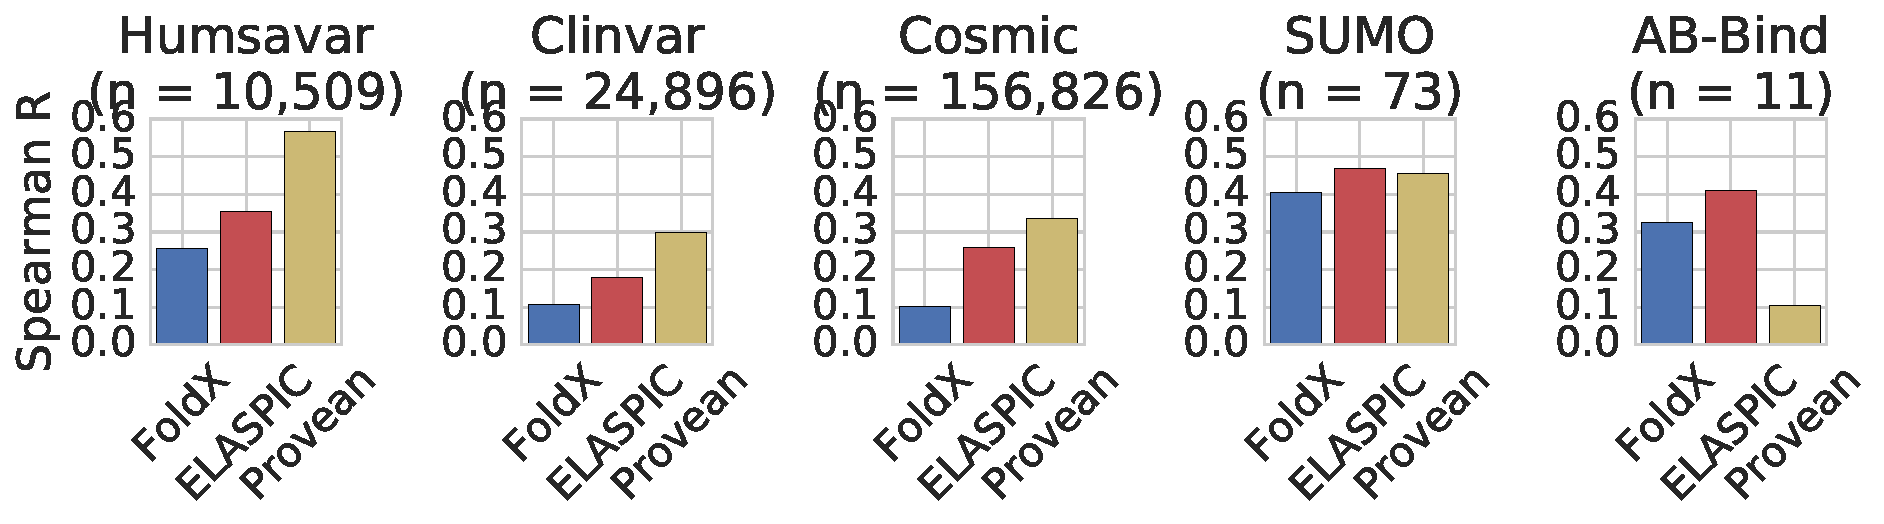
\includegraphics[width=1.0\textwidth]{static/elaspic_training_set/validation/test_performance_core.pdf}
		\caption{
			Performance of the ELASPIC core predictor, FoldX and Provean on the test datasets.
			There is no overlap in mutations (or proteins for Humsavar, ClinVar and COSMIC) between the test datasets,
			and the training and validation datasets (see Figure \ref{fig:training_set_overlap_core}).
		}
		\label{fig:test_performance_core}
		\vspace*{5mm}
	\end{subfigure}
	\caption[Core predictor validation.]{Performance of the ELASPIC core predictor on the training (a), validation (b) and test (c) datasets.}
	\label{fig:core_validation}
\end{figure}

\clearpage

\begin{figure}[tb]
	\centering
	\begin{subfigure}[b]{1.0\textwidth}
		\centering
		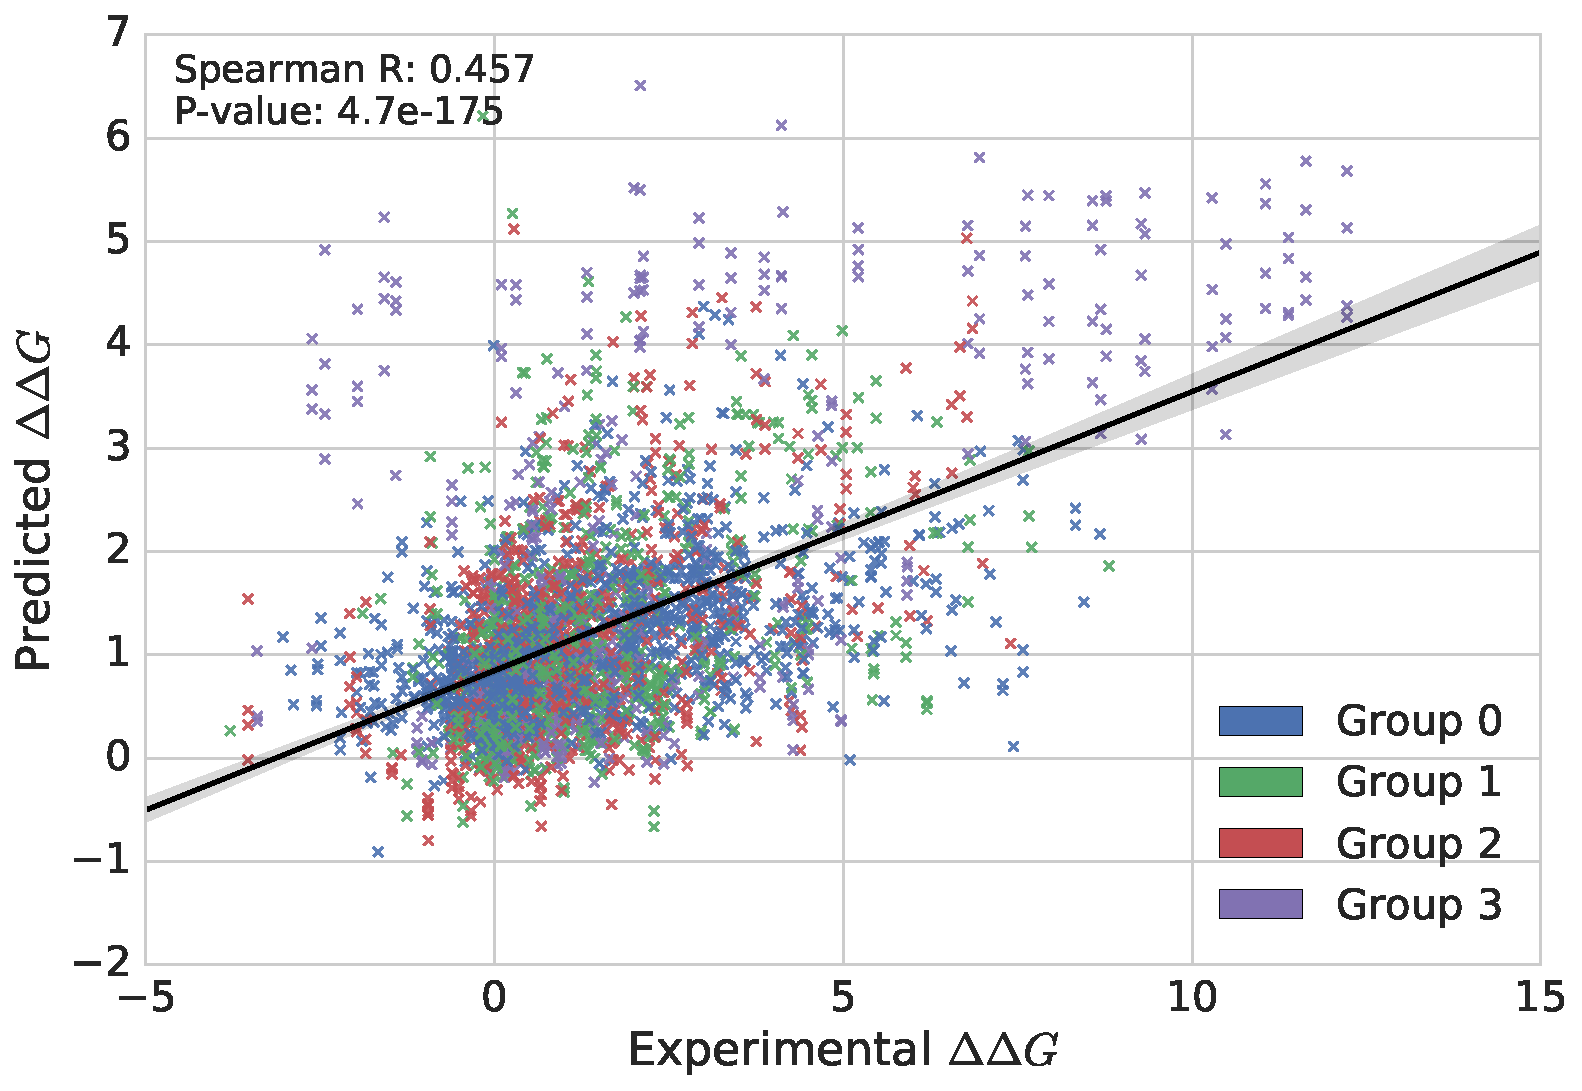
\includegraphics[width=0.6\linewidth]{static/elaspic_training_set/validation/crossvalidation_performance_interface.pdf}
		\caption{
			Performance of the ELASPIC interface predictor on the training dataset, evaluated using four-fold cross-validation.
			Colours indicate different cross-validation bins.
		}
		\label{fig:crossvalidation_performance_interface}
		\vspace*{10mm}
	\end{subfigure}
	\begin{subfigure}[b]{1.0\textwidth}
		\centering
		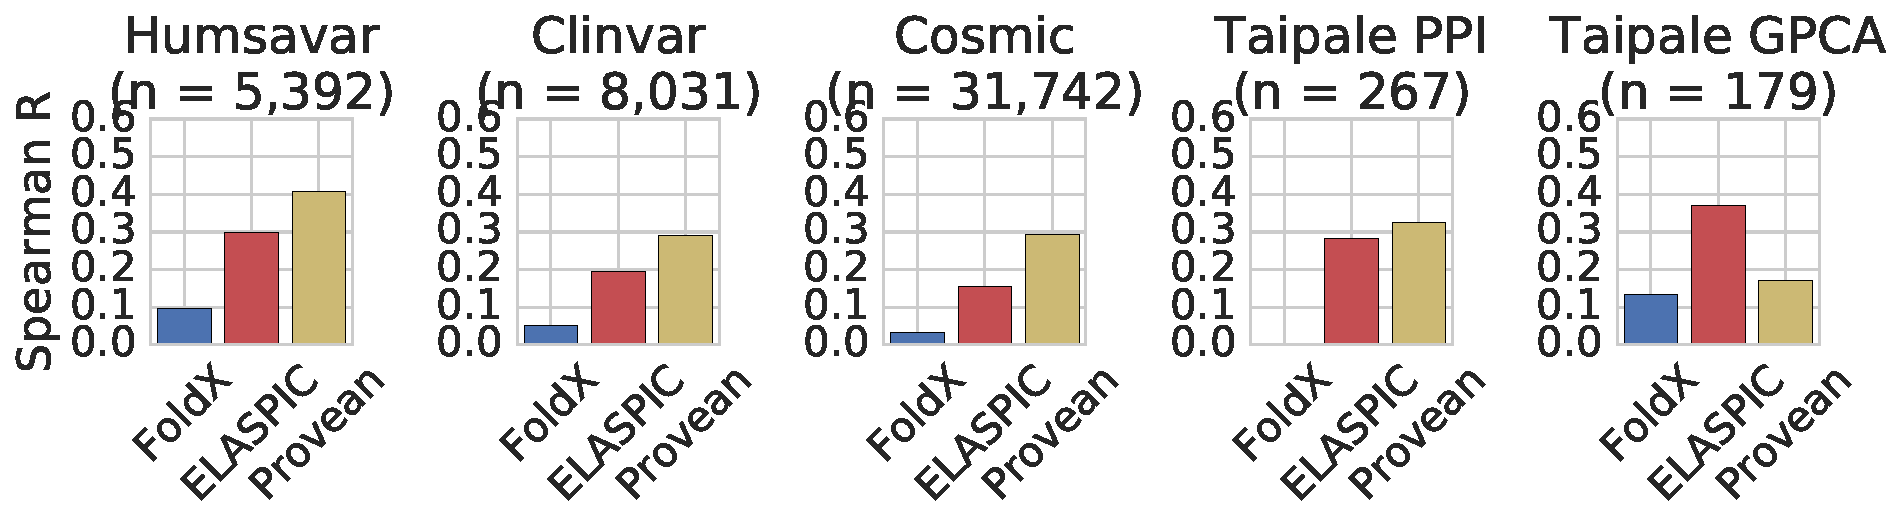
\includegraphics[width=0.9\textwidth]{static/elaspic_training_set/validation/validation_performance_interface.pdf}
		\caption{
			Performance of the ELASPIC interface predictor, FoldX and Provean on the validation datasets.
		}
		\label{fig:validation_performance_interface}
		\vspace*{10mm}
	\end{subfigure}
	\begin{subfigure}[b]{1.0\textwidth}
		\centering
		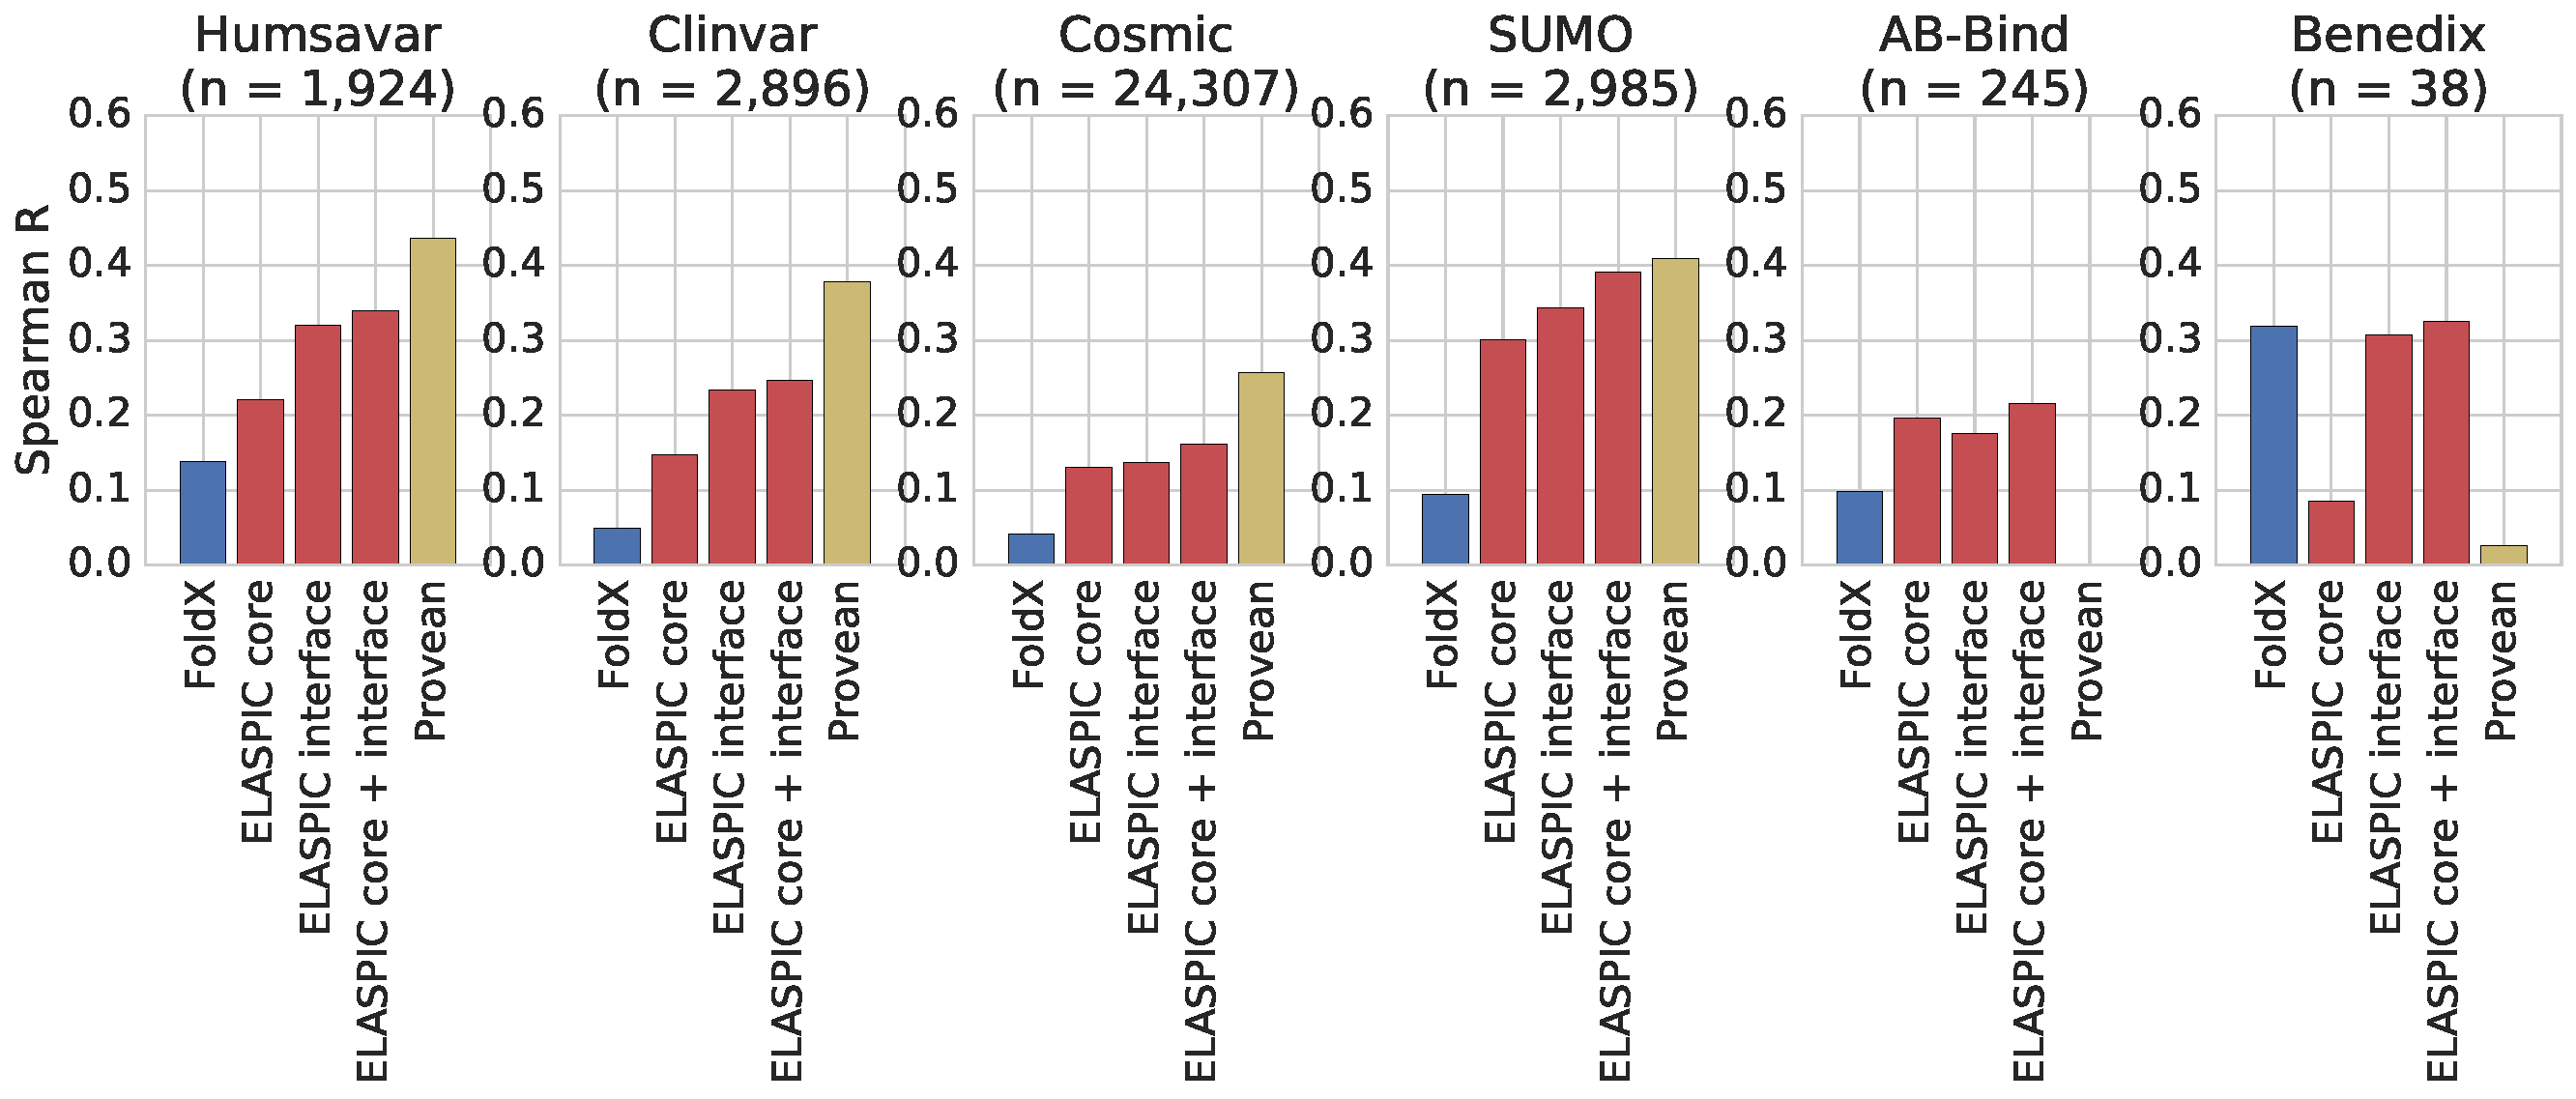
\includegraphics[width=1.0\textwidth]{static/elaspic_training_set/validation/test_performance_interface.pdf}
		\caption{
			Performance of ELASPIC, FoldX and Provean on the test datasets.
			Correlations are provided for core predictor outputs, interface predictor outputs, and the sum of core and interface predictor outputs, for ELASPIC and FoldX.
			There is no overlap in mutations (or proteins for Humsavar, ClinVar and COSMIC) between the test datasets,
			and the training and validation datasets (see Figure \ref{fig:training_set_overlap_interface}).
		}
		\label{fig:test_performance_interface}
		\vspace*{5mm}
	\end{subfigure}
	\caption[Interface predictor validation.]{Performance of the ELASPIC interface predictor on the training (a), validation (b) and test (c) datasets.}
	\label{fig:interface_validation}
\end{figure}
